\documentclass[tikz,border=2pt]{standalone}
% Preámbulo común de los diagramas TikZ (misma paleta y letra que las notas)
\usepackage[T1]{fontenc}\usepackage[utf8]{inputenc}
\usepackage{libertinus}\usepackage{libertinust1math}
\usepackage[defaultsans,scale=0.92]{lato}
\usepackage{amsmath,amssymb,bm}
\usepackage{tikz}\usetikzlibrary{calc,positioning,arrows.meta,shapes.geometric,decorations.pathreplacing,decorations.pathmorphing,fit,backgrounds}
\definecolor{snlazul}{HTML}{1E5AA8}\definecolor{snlnoche}{HTML}{14213D}\definecolor{snlvioleta}{HTML}{6C4AB6}
\definecolor{snlcoral}{HTML}{D1495B}\definecolor{snlambar}{HTML}{E09F3E}\definecolor{snlverde}{HTML}{2A9D8F}
\definecolor{snlteal}{HTML}{0F7173}\definecolor{snlgris}{HTML}{5C677D}\definecolor{snlfondo}{HTML}{F4F6FA}
\tikzset{>={Stealth[length=2.2mm]},
  bloque/.style={draw=#1,fill=#1!8,thick,rounded corners=2pt,minimum height=11mm,minimum width=20mm,align=center,font=\small},
  bloque/.default=snlazul,
  suma/.style={draw=snlnoche,thick,circle,inner sep=0pt,minimum size=5mm},
  flecha/.style={->,thick,draw=snlnoche},
  etq/.style={font=\small,text=snlnoche},
  nota/.style={font=\footnotesize\sffamily,text=snlgris,align=center}}

\begin{document}
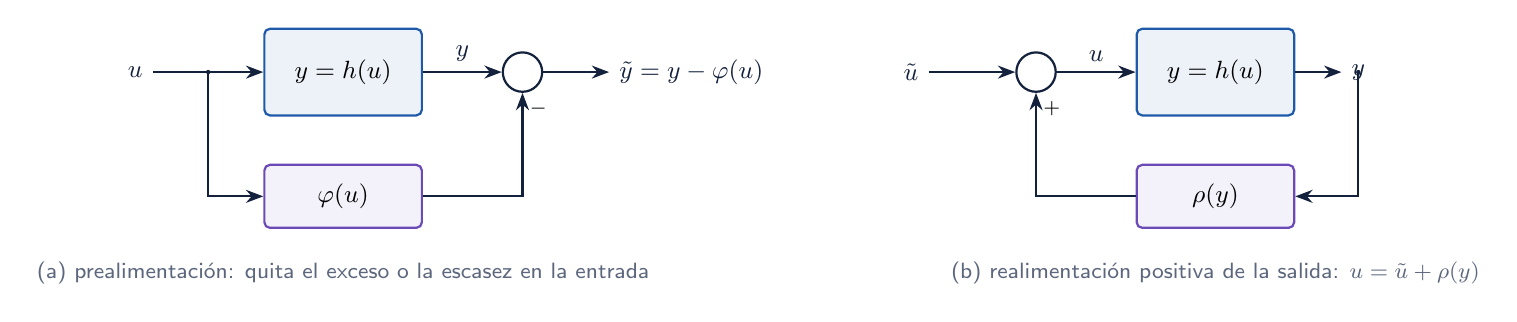
\begin{tikzpicture}
 % (a) prealimentación
 \node[bloque=snlazul] (H) {$y=h(u)$};
 \node[suma,right=10mm of H] (s) {};
 \node[bloque=snlvioleta,below=6mm of H,minimum height=8mm] (phi) {$\varphi(u)$};
 \draw[flecha] ($(H.west)+(-14mm,0)$) node[left,etq]{$u$} -- (H);
 \draw[flecha] (H) -- node[above,etq]{$y$} (s);
 \draw[flecha] ($(H.west)+(-7mm,0)$) |- (phi);
 \fill[snlnoche] ($(H.west)+(-7mm,0)$) circle(0.8pt);
 \draw[flecha] (phi) -| (s);
 \draw[flecha] (s) -- ++(11mm,0) node[right,etq]{$\tilde y=y-\varphi(u)$};
 \node[font=\scriptsize] at ($(s.south)+(2mm,-2mm)$) {$-$};
 \node[nota,below=3mm of phi] {(a) prealimentación: quita el exceso o la escasez en la entrada};
 % (b) realimentación de la salida
 \begin{scope}[xshift=88mm]
 \node[suma] (t) {};
 \node[bloque=snlazul,right=10mm of t] (G) {$y=h(u)$};
 \node[bloque=snlvioleta,below=6mm of G,minimum height=8mm] (rho) {$\rho(y)$};
 \draw[flecha] ($(t.west)+(-11mm,0)$) node[left,etq]{$\tilde u$} -- (t);
 \draw[flecha] (t) -- node[above,etq]{$u$} (G);
 \draw[flecha] (G) -- ++(16mm,0) node[right,etq]{$y$};
 \draw[flecha] ($(G.east)+(8mm,0)$) |- (rho);
 \fill[snlnoche] ($(G.east)+(8mm,0)$) circle(0.8pt);
 \draw[flecha] (rho) -| (t);
 \node[font=\scriptsize] at ($(t.south)+(2mm,-2mm)$) {$+$};
 \node[nota,below=3mm of rho] {(b) realimentación positiva de la salida: $u=\tilde u+\rho(y)$};
 \end{scope}
\end{tikzpicture}
\end{document}
